\documentclass[border=10pt]{standalone}
\usepackage{tikz}
\usepackage{pgfplots}
\pgfplotsset{compat=1.8}

\begin{document}
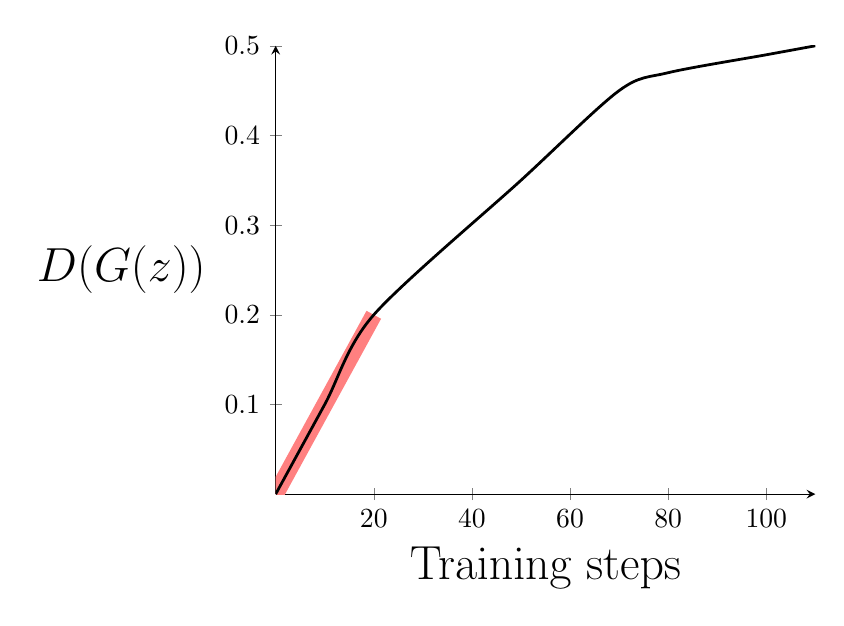
\begin{tikzpicture}
	\begin{axis}[
		xlabel={Training steps},
		axis lines=middle,
		ylabel near ticks,
		xlabel near ticks,
		ylabel={$D(G(z))$},
		ylabel style={rotate=-90, font=\LARGE},
		xlabel style={font=\LARGE}
	]
	
	% shading
	\addplot[line width=6pt,color = red!50, domain = 0:0.2, smooth]
	coordinates {
		(0, 0)
		(10,0.1)
		(20,0.2)};
	
	\addplot [mark=none,domain=0:1, line width=1pt, smooth] coordinates {
		(0, 0)
		(10,0.1)
		(20,0.2)
		(50,0.35)
		(70, 0.45)
		(80, 0.47)
		(100, 0.49)
		(110, 0.5)};

	\end{axis}

\end{tikzpicture}

\end{document}